\documentclass{report}
% Comment the following line to NOT allow the usage of umlauts
\usepackage[utf8]{inputenc}
% Uncomment the following line to allow the usage of graphics (.png, .jpg)

\usepackage{geometry}
\geometry{left=3cm,right=3cm,top=3cm,bottom=3cm}

\usepackage[usenames,dvipsnames]{color}
\usepackage[table,xcdraw]{xcolor}
\usepackage[colorlinks,linkcolor=NavyBlue,citecolor=green, urlcolor=green]{hyperref}


\usepackage{graphicx}
\usepackage{enumerate}
\usepackage{float}
\usepackage{bm}
\usepackage{array,makecell}
\usepackage{multirow}

\usepackage{amsmath,amsfonts}
\usepackage{amssymb}
\usepackage{siunitx}
\usepackage{tabularray}
\usepackage[thmmarks,amsmath]{ntheorem}
\usepackage[all]{xy}
\usepackage{tikz}

\usepackage{quiver}

\theorembodyfont{\upshape}
\newtheorem{definition}{Definition}[section]
\newtheorem{example}{Example}[section]
\newtheorem{proposition}{Proposition}[section]
\newtheorem{theorem}{Theorem}[section]
\newtheorem{lemma}{Lemma}[section]
\theoremstyle{nonumberplain}
\theoremheaderfont{\itshape}
\theorembodyfont{\normalfont}
\theoremsymbol{\\ \rightline{$\square$}}
\newtheorem{proof}{Proof.}

\newcommand{\Top}{\mathsf{Top}}
\newcommand{\Grp}{\mathsf{Grp}}
\newcommand{\Grpd}{\mathsf{Grpd}}
\newcommand{\Obj}{\mathrm{Obj}}
\newcommand{\Hom}{\mathrm{Hom}}

% Start the document
\begin{document}
\begin{center}
	~\\
	\vspace{6em}
	\textsc{\Huge TOPOLOGY}
	~\\
	\vspace{2.5em}
	{\Large }
	~\\
	\vspace{6em}
	\textsf{Huyi Chen}
	~\\
	\vspace{5in}
	{\large Latest Update: \today}
\end{center}
\newpage
\tableofcontents
% Create a new 1st level heading
\chapter{Preliminaries}

\section{Naive Set Theory}
Suppose that $A_\alpha,A,B_\alpha,B$ are sets and $I$ is some index set. We have
\begin{itemize}
	\item $A\cap\left(\bigcup\limits_{\alpha\in I}B_\alpha\right)=\bigcup\limits_{\alpha\in I}\left(A\cap B_\alpha\right)\ $, $A\cup\left(\bigcap\limits_{\alpha\in I}B_\alpha\right)=\bigcap\limits_{\alpha\in I}\left(A\cup B_\alpha\right)$.
	\item $\left(\bigcup\limits_{\alpha\in I}A_\alpha\right)^C=\bigcap\limits_{\alpha\in I}A_\alpha^{\,C}\ $, $\left(\bigcap\limits_{\alpha\in I}A_\alpha\right)^C=\bigcup\limits_{\alpha\in I}A_\alpha^{\,C}$
	\item $E-\bigcup\limits_{\alpha\in I}A_\alpha=\bigcap\limits_{\alpha\in I}\left(E-A_\alpha\right)\ $, $E-\bigcap\limits_{\alpha\in I}A_\alpha=\bigcup\limits_{\alpha\in I}\left(E-A_\alpha\right)\ $
\end{itemize}
Let $f:X\to Y$ be a map. Suppose that $A_\alpha,A,E\subset X$ and $B_\alpha,B,F\subset Y$. We have
\begin{itemize}
	\item $f\left(\bigcup\limits_{\alpha\in I}A_\alpha\right)=\bigcup\limits_{\alpha\in I}f\left(A_\alpha\right)\ $, $f\left(\bigcap\limits_{\alpha\in I}A_\alpha\right)\subset\bigcap\limits_{\alpha\in I}f\left(A_\alpha\right)\ $, $f(E-A)\supset f(E)-f(A)$.
	\item $f^{-1}\left(\bigcup\limits_{\alpha\in I}B_\alpha\right)=\bigcup\limits_{\alpha\in I}f^{-1}\left(B_\alpha\right)\ $, $f^{-1}\left(\bigcap\limits_{\alpha\in I}B_\alpha\right)=\bigcap\limits_{\alpha\in I}f^{-1}\left(B_\alpha\right)\ $, $f^{-1}(F-B)=f^{-1}(F)-f^{-1}(B)$.
	\item $A\subset f^{-1}(f(A))\ $, $B\supset f(f^{-1}(B))$.
\end{itemize}

\chapter{General Topology}
\section{Topological space}

\begin{definition}[topological space]
	A \emph{topological space} is an ordered pair $(X,\tau)$, where $X$ is a set and $\tau\subset\mathcal{P}(X)$ is a collection of subsets of $X$, satisfying the following axioms:
	\begin{enumerate}
		\item $\varnothing\in \tau$, $X\in \tau$.
		\item If $A_i\in\tau\;(i\in I)$, then $\bigcup\limits_{i\in I}A_i\in \tau$,
		\item If $A_i\in\tau\;(i=1,2,\cdots,n)$, then $\bigcap\limits_{i=1}^nA_i\in \tau$.
	\end{enumerate}
	\noindent The elements of $\tau$ are called \emph{open sets} and the collection $\tau$ is called a \emph{topology} on $X$.
\end{definition}

\noindent In this chapter we always assume that $(X,\tau)$ is a topological space.


\begin{definition}[closed set]
	Suppose that $A$ is a subset of $X$. $A$ is a \emph{closed set} if and only if $A^C$ is an open set.
\end{definition}

\begin{proposition}
	Assume that $\mathcal{F}\subset\mathcal{P}(X)$ is a collection of all closed sets of $(X,\tau)$.
	\begin{enumerate}
		\item $\varnothing\in \mathcal{F}$, $X\in \mathcal{F}$.
		\item If $A_i\in\mathcal{F}\;(i\in I)$, then $\bigcap\limits_{i\in I}A_i\in \mathcal{F}$,
		\item If $A_i\in\mathcal{F}\;(i=1,2,\cdots,n)$, then $\bigcup\limits_{i=1}^nA_i\in \mathcal{F}$.
	\end{enumerate}
\end{proposition}
\begin{proof}~\\
	\begin{enumerate}
		\item \vspace{-1em}$\varnothing\in \tau\implies\varnothing^C=X\in \mathcal{F} \ $. $X\in \tau\implies X^C=\varnothing\in \mathcal{F}$.
		\item $A_i\in\mathcal{F}\;(i\in I)\implies A_i^C\in\tau\;(i\in I)\implies\bigcup\limits_{i\in I}A_i^C\in \tau\implies \left(\bigcap\limits_{i\in I}A_i\right)^C\in \tau\implies\bigcap\limits_{i\in I}A_i\in\mathcal{F}$.
		\item $A_i\in\mathcal{F}\;(i=1,\cdots,n)\implies A_i^C\in\tau\;(i=1,\cdots,n)\implies\bigcap\limits_{i=1}^nA_i^C\in \tau\implies \left(\bigcup\limits_{i=1}^nA_i\right)^C\in \tau\implies\bigcup\limits_{i=1}^nA_i\in\mathcal{F}$.
	\end{enumerate}
\end{proof}

\begin{definition}[neighborhood]
	Given a point $x\in X$, a set $N\subset X$ is the \emph{neighborhood} of $x$ if there exists an open set $O\in\tau$ such that $x\in O\subset N$. The collection of all neighborhoods of $x$ is denoted by $\mathcal{N}(x)$.
\end{definition}

\begin{proposition}
	Suppose that $x\in X$.
	\begin{enumerate}
		\item $N\in\mathcal{N}(x)\implies x\in N$
		\item $N_1,N_2\in\mathcal{N}(x)\implies N_1\cap N_2\in\mathcal{N}(x)$
		\item $N\in\mathcal{N}(x)\bigwedge N\subset U\subset X\implies U\in\mathcal{N}(x)$
		\item $N\in\mathcal{N}(x)\implies \exists M\in\mathcal{N}(x),\ (M\subset N)\bigwedge(\,\forall y\in M,M\in\mathcal{N}(y)\hspace{1pt})$
	\end{enumerate}
\end{proposition}
\begin{proof}~\\ \vspace{-1em}
	\begin{enumerate}
		\item $N\in\mathcal{N}(x)\implies x\in O\subset N \implies x\in N$.
		\item $N_1,N_2\in\mathcal{N}(x)\implies x\in O_1\subset N_1 \bigwedge x\in O_2\subset N_2\implies x\in O_1\cap O_2\subset N_1\cap N_2$.
		\item $N\in\mathcal{N}(x)\bigwedge N\subset U\subset X\implies x\in O\subset N\subset U\implies U\in\mathcal{N}(x)$.
		\item If $N\in\mathcal{N}(x)$, then there exists $O\in\tau$ such that $x\in O\subset N$. Note that $O\in \mathcal{N}(x)$ and
		      \[
			      \forall y\in O,y\in O\subset O\implies\forall y\in O,O\in\mathcal{N}(y).
		      \]
		      We affirm that $O$ is the set $M$ that we are looking for.
	\end{enumerate}
\end{proof}
\begin{definition}[limit point]
	Suppose that $A$ is a subset of $X$. A point $x\in X$ is a \emph{limit point} of $A$, if every neighbourhood of $x$ contains at least one point of $A$ different from $x$ itself,
	or alternatively, if for any open set $O$ containing $x$,
	\[
		O\cap(A-\{x\})\ne\varnothing.
	\]
	The set of all limit points of $A$ is said to be the \emph{derived set} of $A$, denoted by $A'$.
\end{definition}

\begin{proposition}
	Suppose that $A$ and $B$ are subsets of $X$.
	\begin{enumerate}
		\item $\varnothing'=\varnothing$
		\item $(A \cup B)'=A'\cup B' $
		\item $A \subset B \Longrightarrow A' \subset B'$
		\item $A'' \subset A' \cup A $
		\item $a \in A' \Longrightarrow a \in(A-\{a\})' $
	\end{enumerate}
\end{proposition}
\begin{proof}~\\ \vspace{-1em}
	\begin{enumerate}
		\item For any point $x\in X$ and for any neighborhood $N\in\mathcal{N}(x)$, we have $N\cap(\varnothing-\{x\})=\varnothing$. It implies that empty set has no limit points.
		\item Omitted.
	\end{enumerate}
\end{proof}

\begin{definition}[closure]
	Suppose that $A$ is a subset of $X$. The \emph{closure} of $A$ is the smallest closed set containing $A$, denoted by $\overline{A}$.
\end{definition}

\begin{proposition}
	The following propositions are equivalent:
	\begin{enumerate}
		\item $S$ is the closure of $A$.
		\item $S=\bigcap\limits_{F_\alpha\in\mathcal{F}:A\subset F_\alpha}F_\alpha$, where $\mathcal{F}$ is a collection of all closed sets of $X$.
		\item $S=A\cup A'$.
		\item $S=\{x\in X: \forall N\in\mathcal{N}(x),N\cap A\ne\varnothing\}$.
	\end{enumerate}
\end{proposition}

\begin{proof}~\\ \vspace{-1em}
	\begin{enumerate}
		\item Omitted.
	\end{enumerate}
\end{proof}
\begin{proposition}
	Suppose that $A$ and $B$ are subsets of $X$.
	\begin{enumerate}
		\item $\overline{\varnothing}=\varnothing$.
		\item $\overline{A \cup B}=\overline{A}\cup\overline{B}$,  $\overline{A \cap B}\subset\overline{A}\cap\overline{B}$.
		\item $A\subset\overline{A}$.
		\item $\overline{\left(\overline{A}\right)}=\overline{A}$.
	\end{enumerate}
\end{proposition}

\begin{proof}~\\ \vspace{-1em}
	\begin{enumerate}
		\item Omitted.
	\end{enumerate}
\end{proof}

\begin{definition}[frontier]
	Suppose that $A$ is a subset of $X$. The \emph{frontier} of $A$ denoted by $\partial A$ is defined as
	\[
		\partial A=\overline{A}\cap\overline{A^C}.
	\] A point $x$ is called an \emph{boundary point} of $A$ if $x\in \partial A$.
\end{definition}

\begin{definition}[interior]
	Suppose that $A$ is a subset of $X$. The \emph{interior} of $A$ is the largest open set contained by $A$, denoted by $A^{\circ}$. A point $x$ is called an \emph{interior point} of $A$ if $x\in A^{\circ}$.
\end{definition}

\begin{proposition}
	The following propositions are equivalent:
	\begin{enumerate}
		\item $S$ is the interior of $A$.
		\item $S=\bigcup\limits_{O_\alpha\in\tau:O_\alpha\subset A}O_\alpha$.
		\item $S=A-\partial A$.
		\item $S=\{x\in X:\exists N\in\mathcal{N}(x),N_x\subset A\}$.
	\end{enumerate}
\end{proposition}
\begin{proof}~\\ \vspace{-1em}
	\begin{enumerate}
		\item Omitted.
	\end{enumerate}
\end{proof}
\begin{proposition}
	Suppose that $A$ and $B$ are subsets of $X$.
	\begin{enumerate}
		\item $\varnothing^{\circ}=\varnothing$.
		\item $(A \cup B)^{\circ}=A^{\circ}\cup B^{\circ}$,  $(A \cap B)^{\circ}\supset A^{\circ}\cap B^{\circ}$.
		\item $A\supset A^{\circ}$.
		\item $\left(A^{\circ}\right)^{\circ}=A^{\circ}$.
	\end{enumerate}
\end{proposition}

\begin{proof}~\\ \vspace{-1em}
	\begin{enumerate}
		\item Omitted.
	\end{enumerate}
\end{proof}

\begin{proposition}
	The following propositions are equivalent:
	\begin{enumerate}
		\item $F$ is a closed set.
		\item $F'\subset F$.
		\item $\overline{F}=F$.
	\end{enumerate}
\end{proposition}
\begin{proof}~\\ \vspace{-1em}
	\begin{enumerate}
		\item Omitted.
	\end{enumerate}
\end{proof}

\begin{proposition}
	The following propositions are equivalent:
	\begin{enumerate}
		\item $F$ is an open set.
		\item $\partial F\cap F=\varnothing$.
		\item $F^\circ=F$.
		\item $\forall x\in F,F\in \mathcal{N}(x)$.
	\end{enumerate}
\end{proposition}
\begin{proof}~\\ \vspace{-1em}
	\begin{enumerate}
		\item Omitted.
	\end{enumerate}
\end{proof}

\begin{proposition}
	Suppose that $A$ is a subset of $X$.
	\begin{enumerate}
		\item $(\overline{A})^C=(A^C)^{\circ}$
		\item $(A^{\circ})^C=\overline{A^C}$
	\end{enumerate}
\end{proposition}
\begin{proof}~\\ \vspace{-1em}
	\begin{enumerate}
		\item Omitted.
	\end{enumerate}
\end{proof}

\begin{definition}[dense set]
	A subset $A$ of a topological space $X$ is called dense in $X$ if  $\overline{A}=X$.
\end{definition}
\begin{proposition}
	The following propositions are equivalent:
	\begin{enumerate}
		\item $A$ is dense in $X$.
		\item For any point $x \in X$ and for any neighborhood $N\in\mathcal{N}(x)$, $N\cap A\ne \varnothing$.
	\end{enumerate}
\end{proposition}
\begin{proof}~\\ \vspace{-1em}
	\begin{enumerate}
		\item Omitted.
	\end{enumerate}
\end{proof}

\begin{definition}
	Let $\mathcal{B}$ is a collection of subsets of $X$, the collection of subsets generated by $\mathcal{B}$ is defined as
	\[
		\langle\mathcal{B}\rangle=\left\{A\in 2^X:A=\bigcup_{i\in I} B_i,B_i\in\mathcal{B}\right\}.
	\]
\end{definition}
\begin{definition}[base]
	Let $\mathcal{B}$ be a collection of subsets of the topological space $(X,\tau)$. $B$ is a \emph{base} for $(X,\tau)$ if
	$\langle\mathcal{B}\rangle=\tau$.
\end{definition}
\begin{proposition}
	Let $\mathcal{B}$ be a collection of subsets of the topological space $(X,\tau)$. The following propositions are equivalent:
	\begin{enumerate}
		\item $\mathcal{B}$ is a base for $X$.
		\item Elements in $\mathcal{B}$ cover $X$ and $\forall B_1,B_2\in\mathcal{B}$, $\forall x\in B_1\cap B_2$, $\exists B_3\in B_1\cap B_2$ such that $x\in B_3$.
	\end{enumerate}
\end{proposition}


\begin{definition}[separable space]
	A topological space is called \emph{separable} if it contains a countable, dense subset.
\end{definition}

\begin{definition}[second-countable space]
	A \emph{second-countable} space, also called a completely separable space, is a topological space whose topology has a countable base.
\end{definition}

We have several separation axioms in topological spaces denoted by $\mathrm{T}_r$, $r=0,1,2,2\frac{1}{2},3,3\frac{1}{2},4,5,6$.
\begin{definition}[Hausdorff space/$\mathrm{T}_2$ space]
	A topological space $X$ is a \emph{Hausdorff space}, separated space or $\mathrm{T}_2$ space if for any two distinct points $x,y\in X$ there exists a neighbourhood $U$ of $x$ and a neighbourhood $V$ of $y$ such that $U\cap V=\varnothing$.
\end{definition}
\begin{definition}[normal space/$\mathrm{T}_4$ space]
	A topological space $X$ is a \emph{normal space} or $\mathrm{T}_4$ space if, given any disjoint closed sets $E$ and $F$ in $X$, there are neighbourhoods $U$ of $E$ and $V$ of $F$ such that $U\cap V=\varnothing$.
\end{definition}

A subset $K$ of a topological space $X$ is said to be compact if it is compact as a subspace (in the subspace topology).
\section{Basic Construction}
\subsection{Subspace Topology}
\begin{definition}[subspace topology]
	Let $(X,\tau)$ be a topological space and $Y$ be a subset of $X$. Then
	\[
		\tau_Y:=\{Y\cap U\mid U\in \tau\}.
	\]
	is said to be a \emph{subspace topology} of $(X,\tau)$.
\end{definition}
$(Y,\tau_Y)$ is a topological space. Moreover, $(Y,\tau_Y)$ is a subobject of $(X,\tau)$ in $\Top$. 

\subsection{Quotient Topology}
\begin{definition}[quotient space]
	Let $(X,\tau)$ be a topological space and $\sim$ be a equivalence relation on $X$. Let $\pi:X\to X/\sim$ be the projection.
	The \emph{quotient space} of $X$ is the set $X/\sim$ equiped with the following topology
	\[
		\tau_\sim:=\{A\in 2^{X/\sim}\mid \pi^{-1}(A)\in \tau\},
	\]
	which is called \emph{quotient topology}.
\end{definition}

It is easy to check that $\pi$ is a continuous surjection from $(X,\tau)$ to $(X/\sim\,,\tau_\sim)$.

\begin{proposition}
	For any topological space $(Y,\sigma)$ and any continuous mapping $f:X\to Y$ such that $a\sim b$ implies $f(a) = f(b)$ for all $a,b \in X$, there exists a unique continuous mapping $\bar{f}:X/\sim\;\to Y$ such that the following diagram commutes.

	\[\xymatrix{
		X\ar[r]^{f\quad}\ar[d]_{\pi}  &Y\\
		X/\sim\ar@{-->}[ru]_{\exists!\bar{f}}&
		}\]
\end{proposition}


\begin{proof}
	Define
	\begin{align*}
		\bar{f}:X/\sim & \longrightarrow Y, \\
		[x]            & \longmapsto f(x).
	\end{align*}
	It is clear that $\bar{f}$ is well-defined. Since for all $B\in \sigma$,
	\[
		\pi^{-1}\left(\bar{f}^{-1}(B)\right)=\pi^{-1}\left(\{[x]\in X/\sim| f(x)\in B\}\right)=\{x\in X| f(x)\in B\}=f^{-1}(B)\in \tau,
	\]
	we have
	\[
		\bar{f}^{-1}(B)\in \tau_\sim,
	\]
	which implies $\bar{f}$ is continuous. If there exists a function $g:X/\sim\;\to Y$ such that $f=g\circ\pi$, then for all $[x]\in X/\sim$, we see
	\[
		g([x])=g(\pi(x))=f(x)\implies g=\bar{f}.
	\]
\end{proof}


\subsection{Product Topology}
\section{Connectedness}

\section{Compactness}
\begin{definition}[compact topological space]
	Formally, a topological space $X$ is called \emph{compact} if each of its open covers has a finite subcover. That is, $X$ is compact if for every collection $\mathcal{C}$ of open subsets of $X$ such that
	\[
		X=\bigcup_{C \in \mathcal{C}} C
	\]
	there is a finite subset $\mathcal{F}$ of $\mathcal{C}$ such that
	\[
		X=\bigcup_{F \in \mathcal{F}} F
	\]
\end{definition}

\chapter{Basic Notions}
\section{CW Complex}
A $k$-cell is a $k$-dimensional disc
\[
	D^k=\{x\in\mathbf{R}^k:\ |x|\leq 1\}.
\]

\chapter{Fundamental Groupoid}
\section{Homotopy}
\begin{definition}[path]	
	A \emph{path} in a topological space $X$ is defined as a continuous function $p:[0,1]\to X$. $p$ is said to be from $x$ to $y$ if $p(0)=x$ and $p(1)=y$.
\end{definition}
We say a path is a \emph{loop} if $p(0)=p(1)$.
\begin{definition}[homotopy]
	A \emph{homotopy} between two continuous functions $f$ and $g$ from a topological space $X$ to a topological space $Y$ is defined to be a continuous function $h: X \times[0,1] \rightarrow Y$ such that $h(x, 0)=f(x)$ and $H(x, 1)=g(x)$ for all $x \in X$.
\end{definition}
\begin{definition}[relative homotopy]
	Let $h: X \times[0,1] \rightarrow Y$ be a homotopy from $f:X\to Y$ to $g:X\to Y$ and $K$ be a subset of $X$. We say $h$ is \emph{homotopy relative to $K$} if $h(k, t)=f(k)=g(k)$ for all $k \in K$ and $t \in[0,1]$. 
\end{definition}
\begin{definition}[homotopy rel end points]
	Let $x,y$ be two points in a topological space $X$. If $p:[0,1]\to X$ and $q:[0,1]\to X$ are two paths from $x$ to $y$, then a \emph{homotopy rel end points from $p$ to $q$} is defined as a homotopy relative to $\{x, y\}$ from $p$ to $q$.
\end{definition}
\begin{definition}[equivalent paths]
	Let $X$ be a topological space. Suppose $f: [0,1] \longrightarrow X$ is a path from $x$ to $y$ are \emph{equivalent} if they are homotopic rel end points. That is, there must exist a homotopy $h: [0,1] \times [0,1] \longrightarrow X$ such that
	$$
	h(s, 0)=f(s), \quad h(s, 1)=g(s), \quad h(0, t)=x, \quad h(1, t)=y
	$$
	for all $s,t \in [0,1]$. Write $[f]$ for the equivalence class of $f$. Write $f\sim g$ if $f$ is equivalent to $g$.
\end{definition}

\begin{definition}[composition of paths]
	Let $x,y,z$ be $3$ points in a topological space $X$. Suppose $f: [0,1] \longrightarrow X$ is a path from $x$ to $y$ and $g: [0,1] \longrightarrow X$ is a path from $y$ to $z$. The \emph{composition of path $f$ and $g$} denoted by $g\cdot f$ is defined to be a path from $x$ to $z$ as follows
	\begin{align*}
		g\cdot f:[0,1] &\longrightarrow X\\
		t &\longmapsto \begin{cases}
			f(2t)&\text{if }t\in\left[0,\frac{1}{2}\right],\\
			g(2t-1)&\text{if }t\in\left(\left.\frac{1}{2},1\right]\right. .
		\end{cases}
	\end{align*}
\end{definition}
\begin{definition}[composition of equivalent classes of paths]
	Suppose $f: [0,1] \longrightarrow X$ is a path from $x$ to $y$ and $g: [0,1] \longrightarrow X$ is a path from $y$ to $z$. The \emph{composition of $[f]$ and $[g]$} denoted by $[g]\cdot [f]$ is defined as follows
	\[
		[g]\cdot [f]:=[g\cdot f].
	\]
\end{definition}
\begin{proof}
	We will show that the composition of equivalent classes of paths is well-defined, namely 
	\[
		f_1\sim f_2,\;g_1\sim g_2\implies [g_1\cdot f_1] = [g_2\cdot f_2].
	\]
	Suppose $f_1\sim f_2$, $g_1\sim g_2$, $h_f$ is a homotopy rel end points from $f_1$ to $f_2$, and $h_g$ is a homotopy rel end points from $g_1$ to $g_2$. Then
	\begin{align*}
		h_g\cdot h_f:[0,1]\times [0,1] &\longrightarrow x\\
		(s,t) &\longmapsto \begin{cases}
			h_f(2s, t)&\text{if }s\in\left[0,\frac{1}{2}\right],\\
			h_g(2s-1, t)&\text{if }s\in\left(\left.\frac{1}{2},1\right]\right.
		\end{cases}
	\end{align*}
	is a homotopy rel end points from $g_1\cdot f_1$ to $g_2\cdot f_2$, because for all $s\in[0,1]$,
	\begin{align*}
		\left(h_g\cdot h_f\right)(s, 0)=\begin{cases}
			h_f(2s, 0)&\text{if }s\in\left[0,\frac{1}{2}\right],\\
			h_g(2s-1, 0)&\text{if }s\in\left(\left.\frac{1}{2},1\right]\right.
		\end{cases}=\begin{cases}
			f_1(2s)&\text{if }s\in\left[0,\frac{1}{2}\right],\\
			g_1(2s-1)&\text{if }s\in\left(\left.\frac{1}{2},1\right]\right.
		\end{cases}=\left(g_1\cdot f_1\right)(s),\\
		\left(h_g\cdot h_f\right)(s, 1)=\begin{cases}
			h_f(2s, 1)&\text{if }s\in\left[0,\frac{1}{2}\right],\\
			h_g(2s-1, 1)&\text{if }s\in\left(\left.\frac{1}{2},1\right]\right.
		\end{cases}=\begin{cases}
			f_2(2s)&\text{if }s\in\left[0,\frac{1}{2}\right],\\
			g_2(2s-1)&\text{if }s\in\left(\left.\frac{1}{2},1\right]\right.
		\end{cases}=\left(g_2\cdot f_2\right)(s).
	\end{align*}
	Thus we have $g_1\cdot f_1\sim g_2\cdot f_2$, which implies $\cdot$ is well-defined.
	Suppose $f_1\sim f_2$, $h$ is a homotopy rel end points from $f_1$ to $f_2$. Then

\end{proof}
\begin{definition}[inverse of path]
	Let $p: [0,1] \longrightarrow X$ is a path from $x$ to $y$. The \emph{inverse of path $p$} denoted by $p^{-1}$ is defined to be a path from $y$ to $x$ as follows
	\begin{align*}
		p^{-1}:[0,1]&\longrightarrow X\\
		s &\longmapsto p(1-s).
	\end{align*}
\end{definition}
\begin{definition}[inverse of equivalent class of paths]
	Let $X$ be a topological space and $p:[0,1]\to X$ be a path. Then the \emph{inverse of path $p$} denoted by $[p]^{-1}$ is defined as follows
	\begin{align*}
		[p]^{-1}:=[p^{-1}].
	\end{align*}
\end{definition}
\begin{proof}
	We will show that the inverse of equivalent classes of paths is well-defined, namely 
	\[
		p_1\sim p_2\implies [p_1]^{-1} = [p_2]^{-1}.
	\]
	Suppose $p_1\sim p_2$ and $h$ is a homotopy rel end points from $p_2$ to $p_2$. Then $r(s,t):=h(1-s, t)$
	is a homotopy rel end points from $p_1^{-1}$ to $p_2^{-1}$, because for all $s\in[0,1]$,
	\begin{align*}
		r(s,0)&=h(1-s,0)=p_1(1-s)=p_1^{-1}(s),\\
		r(s,1)&=h(1-s,1)=p_2(1-s)=p_2^{-1}(s).
	\end{align*}
	Thus we have $p_1^{-1}\sim p_2^{-1}$, which implies $[p]^{-1}$ is well-defined.
\end{proof}
\begin{definition}[fundamental group]
	Given a topological space $X$ and a point $x\in X$, define $\pi_1(X, x)$ to be the set of equivalence classes of loops that start and end at $x$. $(\pi_1(X, x),\cdot)$ is a group, called the fundamental group of $X$, where the group operation $\cdot$ is defined as $[g]\cdot[f]:=[g\cdot f]$.
\end{definition}
\begin{proof}
	First we will show that $\cdot$ is associative, that is, $[h]\cdot\left([g]\cdot[f]\right)=\left([h]\cdot[g]\right)\cdot[f]$ or equivalently $[h\cdot(g\cdot f)]=[(h\cdot g)\cdot f]$. It is sufficient to show that $h\cdot(g\cdot f)\sim (h\cdot g)\cdot f$. Define $H:[0,1]\times[0,1]\to X$ as
	\[
		H(s,t)=\begin{cases}
			f\left(\frac{4s}{t+1}\right)&\text{if }s\in\left[0,\frac{t+1}{4}\right],\\
			g(4s-t-1)&\text{if }s\in\left(\left.\frac{t+1}{4},\frac{t+2}{4}\right]\right.,\\
			h\left(\frac{4s-t-2}{2-t}\right)&\text{if }s\in\left(\left.\frac{t+2}{4},1\right]\right.,
		\end{cases}
	\]
	which can be illustrated as follows.
	\begin{center}
		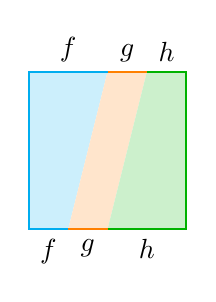
\begin{tikzpicture}
			\path [fill=cyan!20] (0,1)--(-1,1)--(-1,-1)--(-0.5,-1);
			\path [fill=orange!20] (0.5,1)--(0,1)--(-0.5,-1)--(0,-1);
			\path [fill=black!30!green!20] (0.5,1)--(0,-1)--(1,-1)--(1,1);

			\draw [color=cyan, thick] (-0.5,-1)
				-- node [color=black, pos=0.5, below]{$f$} (-1,-1) 
				-- (-1,1)
				-- node [color=black, pos=0.5, above]{$f$} (0,1);

			\draw [color=orange, thick] (-0.5,-1) 
				-- node [color=black, pos=0.5, below]{$g$} (0,-1);
			\draw [color=orange, thick] (0,1) 
				-- node [color=black, pos=0.5, above]{$g$} (0.5,1);

			\draw [color=black!30!green, thick] (0,-1) 
				-- node [color=black, pos=0.5, below]{$h$} (1,-1)
				-- (1,1)
				-- node [color=black, pos=0.5, above]{$h$} (0.5,1);		
		\end{tikzpicture}
	\end{center}
	We can check that $H(s,t)$ is a homotopy rel end points from $h\cdot(g\cdot f)$ to $(h\cdot g)\cdot f$.

	Define a path
	\begin{align*}
		c_x:[0,1] &\longrightarrow X\\
		s &\longmapsto x
	\end{align*}
	We can show that $c_x\cdot f\sim f$ and $f\cdot c_x\sim f$, which means $[c_x]$ is the identity of the group $\pi_1(X,x)$. 

	Given any $[f]\in \pi_1(X,x)$, it is easy to check $\left[f\right]^{-1}\in \pi_1(X,x)$ and $[f]^{-1}\cdot[f]=[f]\cdot[f]^{-1}=[c_x]$.
\end{proof}
\begin{definition}[fundamental groupoid]
	Let $X$ be a topological space. Define $\Pi_1(X)$ to a category, where $\Obj(\Pi_1(X))=X$ and $\Hom_{\Pi_1(X)}(x,y)=\{[f]\mid f:[0,1]\to X \text{ is a path from $x$ to $y$}\}$. $\Pi_1(X)$ is a groupoid and called the fundamental groupoid of $X$.
\end{definition}
\begin{definition}[fundamental groupoid functor]
	Define $\Pi_1:\Top\to\Grpd$ as follows
	\[\begin{tikzcd}
		X & {\Pi_1(X)}\\
		Y & {\Pi_1(Y)} 
		\arrow["f"', from=1-1, to=2-1]
		\arrow["{\Pi_1(f):=[p]\mapsto[f\circ p]}", from=1-2, to=2-2]
		\arrow[from=1-1, to=1-2]
		\arrow[from=2-1, to=2-2]
	\end{tikzcd}\]
\end{definition}
\begin{proof}
	First, we will show that $\Pi_1(f)$ is well-defined, namely for any two paths $p_1$ and $p_2$ in $X$,
	\[
		p_1\sim p_2 \implies [f\circ p_1] = [f\circ p_2].
	\]
	Suppose $p_1\sim p_2$ and $h$ is a homotopy rel end points from $p_2$ to $p_2$. Then $r(s,t):=f(h(s, t))$
	is a homotopy rel end points from $f\circ p_1$ to $f\circ p_2$, because for all $s\in[0,1]$,
	\begin{align*}
		r(s,0)&=f(h(s,0))=f(p_1(s))=f\circ p_1(s),\\
		r(s,1)&=f(h(s,1))=f(p_2(s))=f\circ p_2(s).
	\end{align*}
	Thus we have $f\circ p_1\sim f\circ p_2$, which implies $\Pi_1(f)$ is well-defined.
	To verify the functinality of $\Pi_1$, we have to show that
	\[
		\Pi_1(g\circ f) = \Pi_1(g)\circ\Pi_1(f),
	\]
	or equivalently for all $[p]\in \Pi_1(X)$,
	\[
		[(g\circ f)\circ p]=[g\circ (f\circ p)],
	\]
	which clearly holds. 
\end{proof}




\chapter{Concrete Examples}
A topological space $X$ is called locally Euclidean if there is a non-negative integer $n$ such that every point in $X$ has a neighbourhood which is homeomorphic to real n-dimensional space $\mathbb{R}^n$.

\indent A topological manifold is a locally Euclidean Hausdorff space. In this chapter we focus on some concrete topological manifolds to develop a topological intuition. Topological manifold will be called manifold in brief whenever we mention it.

\section{One-dimensional manifolds}
\subsection{Real affine line $\mathbb{R}^1$}
The real line $\mathbb{R}^1$ carries a standard topology, which can be introduced from the metric defined above. The real line is homeomorphic to any open interval $(a, b)\in\mathbb{R}$.
\begin{center}
	\begin{tikzpicture}
		\path (-4,0.5) node (name1) {$\mathbb{R}^1$};
		\path (4,0.5) node (name2) {$(a,b)$};
		\draw (-6,0) -- (-2,0);
		\draw (name1);
		\draw (0,0) node {$\cong$};
		\draw (2,0) circle [radius=2pt] (2.05,0)-- (5.95,0)(6,0) circle [radius=2pt];
		\draw (name2);
	\end{tikzpicture}
\end{center}
One homeomorphic mapping is
\begin{align*}
	f:\mathbb{R}^1\longrightarrow(a, b),\qquad
	x\longmapsto \frac{b-a}{\pi}\arctan\left(x\right)+\frac{a+b}{2}.
\end{align*}

\subsection{Circle $S^1$}
The circle $S^1$ is defined by $S^1=\{(x,y)\in\mathbb{R}^2|x^2+y^2=1\}$. $S^1$ can be described as $S^1\cong \mathbb{R}^1\cup\{\infty\}$, which is real line plus a single point representing infinity in both directions. Therefore, if a single point $P$ is removed from a circle, it becomes homeomorphic to $\mathbb{R}^1$.
\begin{center}
	\begin{tikzpicture}
		\path (3,0.25) node (name1) {$\mathbb{R}^1$};
		\path (1.1,0.75) node (name2) {$S^1$};
		\draw (0,0) circle [radius=1cm];
		\draw (-4,0) -- (4,0) ;
		\draw[dashed] (0,1) -- (0.5,-0.866025) ;
		\draw (0,1.3) node {$P(\infty)$} ;
		\draw (0,1) circle [radius=2pt] ;
	\end{tikzpicture}
\end{center}
This homeomorphism is exactly the stereographic projection of $P$. Take $P=(0,1)$ and the stereographic projection is given by
\begin{align*}
	pr:S^1-P\longrightarrow \mathbb{R}^1,\qquad      & (x, y) \longmapsto X=\frac{x}{1-y},                                           \\
	pr^{-1}:\mathbb{R}^1\longrightarrow S^1-P,\qquad & X \longmapsto(x, y)=\left(\frac{2X}{X^{2}+1}, \frac{X^{2}-1}{X^{2}+1}\right).
\end{align*}

\subsection{Real projective line $P^1(\mathbb{R})$}
Real projective line $P^1(\mathbb{R})$ is the set of equivalence classes of $\mathbb{R}^2-{(0,0)}$ under the equivalence relation $\sim$ defined by $x\sim y$ if there is a nonzero real number $\lambda$ such that $x = \lambda y$. Given any representative element $(x,y)\in \mathbb{R}^2-{(0,0)}$, the equivalence class of $(x,y)$ is denoted in the form of homogeneous coordinates $[x:y]$. Clearly we have $[x:y]=[\lambda x:\lambda y]$ for any nonzero $\lambda\in \mathbb{R}$.

\indent Real projective line consists of all 1-dimensional subspace of $\mathbb{R}^2$.
\begin{center}
	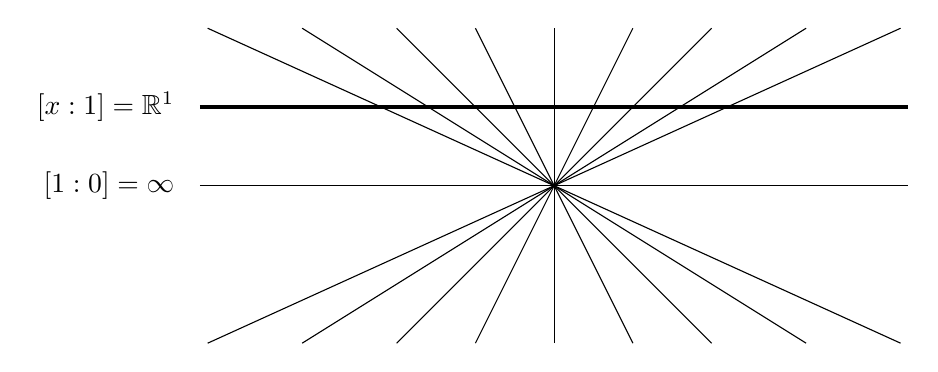
\begin{tikzpicture}
		\draw[very thick] (-4.5,1) -- (4.5,1) ;
		\draw (-4.5,0) -- (4.5,0) ;
		\draw (0,-2) -- (0,2);
		\draw (-2,-2) -- (2,2);
		\draw (-3.2,-2) -- (3.2,2);
		\draw (-1,-2) -- (1,2);
		\draw (2,-2) -- (-2,2);
		\draw (3.2,-2) -- (-3.2,2);
		\draw (1,-2) -- (-1,2);
		\draw (4.4,2) -- (-4.4,-2);
		\draw (4.4,-2) -- (-4.4,2);
		\draw (-4.7,1) node[left] {$[x:1]=\mathbb{R}^1$};
		\draw (-4.7,0) node[left] {$[1:0]=\infty$};
	\end{tikzpicture}
\end{center}
By introduce the continuous mapping
\begin{align*}
	r:P^1(\mathbb{R}) & \longrightarrow\mathbb{R}^1\cup\{\infty\}, \\
	[x:y]             & \longmapsto \frac{x}{y},
\end{align*}
we can clearly see $P^1(\mathbb{R})\cong S^1$.
$P^1(\mathbb{R})$ can be constructed by identifying the antipodal points of $S^1$.
\begin{center}
	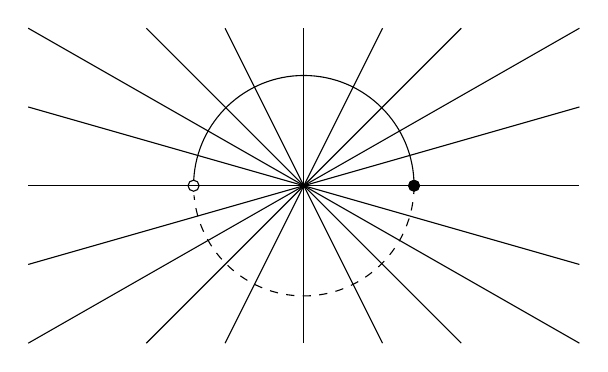
\begin{tikzpicture}
		\draw (1.4,0) arc [start angle=0, end angle=177, radius=1.4cm];
		\draw[dashed] (1.4,0) arc [start angle=0, end angle=-175, radius=1.4cm];
		\draw (-3.5,0) -- (3.5,0) ;
		\draw (0,-2) -- (0,2);
		\draw (-2,-2) -- (2,2);
		\draw (-3.5,-2) -- (3.5,2);
		\draw (-1,-2) -- (1,2);
		\draw (2,-2) -- (-2,2);
		\draw (3.5,-2) -- (-3.5,2);
		\draw (1,-2) -- (-1,2);
		\draw (3.5,1) -- (-3.5,-1);
		\draw (3.5,-1) -- (-3.5,1);
		\draw (-1.4,0) circle [radius=2pt];
		\filldraw (1.4,0) circle [radius=2pt];
	\end{tikzpicture}
\end{center}

\section{Two-dimensional manifolds}
\subsection{Real affine plane $\mathbb{R}^2$}
The real affine plane $\mathbb{R}^2$ carries a standard topology. $\mathbb{R}^2$ is homeomorphic to any open region $G\in\mathbb{R}$.
Since the mapping $(x,y)\mapsto x+\mathrm{i}y$ is a homeomorphism, we have $\mathbb{R}^2\cong \mathbb{C}$.

\subsection{Sphere $S^2$}
The circle $S^2$ is defined by $S^2=\{(x,y,z)\in\mathbb{R}^3|x^2+y^2+z^2=1\}$. Similarly we have $S^2\cong \mathbb{R}^2\cup\{\infty\}$ and the stereographic projection of $P=(0,0,1)$
\begin{align*}
	pr:S^2-P\longrightarrow \mathbb{R}^2,\qquad      & (x, y,z) \longmapsto (X,Y)=\left(\frac{x}{1-z}, \frac{y}{1-z}\right),                                                             \\
	pr^{-1}:\mathbb{R}^1\longrightarrow S^1-P,\qquad & (X,Y) \longmapsto(x, y,z)=\left(\frac{2 X}{X^{2}+Y^{2}+1}, \frac{2 Y}{X^{2}+Y^{2}+1}, \frac{X^{2}+Y^{2}-1}{X^{2}+Y^{2}+1}\right).
\end{align*}
Sphere $S^2$ can be described by a square with some edges identified as follows
\begin{center}
	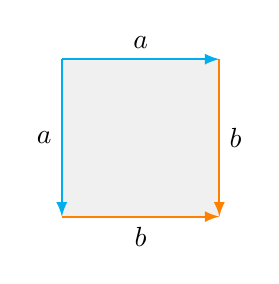
\begin{tikzpicture}
		\fill[fill=gray!12] (-1,-1) --(1,-1)--(1,1)--(-1,1)-- cycle;
		\draw [color=orange,thick,-latex] (-1,-1) -- node [color=black,pos=0.5,below]{$b$} (1,-1);
		\draw [color=cyan,thick,-latex] (-1,1) -- node [color=black,pos=0.5,left]{$a$} (-1,-1);
		\draw [color=orange,thick,-latex] (1,1)--node [color=black,pos=0.5,right]{$b$}(1,-1);
		\draw [color=cyan,thick,-latex] (-1,1)-- node [color=black,pos=0.5,above]{$a$} (1,1);
	\end{tikzpicture}
\end{center}

\subsection{Real projective plane $P^2(\mathbb{R})$}
Real projective plane $P^2(\mathbb{R})=(\mathbb{R}^3-\{(0,0,0)\})/\sim$ where $x\sim y$ whenever there is a nonzero real number $\lambda$ such that $x = \lambda y$. $P^2(\mathbb{R})\cong\mathbb{R}^2\sqcup P^1(\mathbb{R})\cong\mathbb{R}^2\sqcup\mathbb{R}^1\sqcup\{\infty\}$.
\begin{center}
	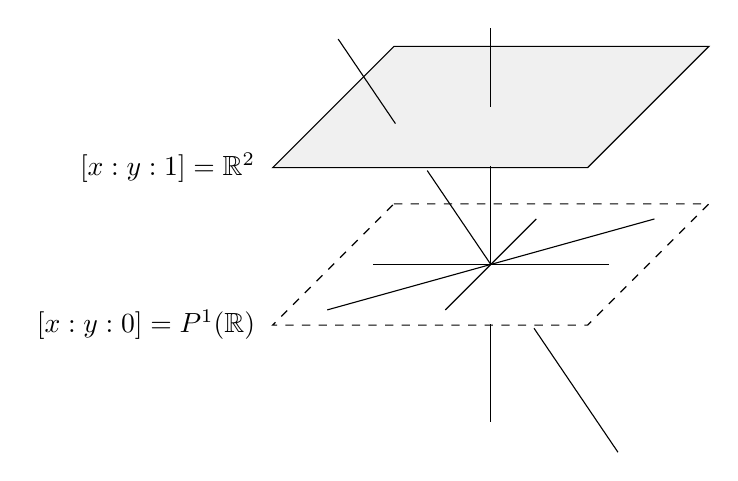
\begin{tikzpicture}
		\draw[dashed] (-2,0,-2) -- (2,0,-2)-- (2,0,2)-- (-2,0,2)--(-2,0,-2);
		\filldraw[fill=gray!12] (-2,2,-2) -- (2,2,-2)-- (2,2,2)-- (-2,2,2)--(-2,2,-2);
		\draw  (1.5,0,-1.5)-- (-1.5,0,1.5);
		\draw  (0,0,-1.5)-- (0,0,1.5);
		\draw  (1.5,0,0)-- (-1.5,0,0);
		\draw (0,-2,0) -- (0,-0.75,0);
		\draw (0,0,0) -- (0,1.25,0);
		\draw (0,2,0) -- (0,3,0);
		\draw (2,-2,1) -- (0.68,-0.68,0.34);
		\draw (0,0,0) -- (-1,1,-0.5);
		\draw (-1.5,1.5,-0.75) -- (-2.4,2.4,-1.2);
		\draw (-2.1,0,2) node[left]{$[x:y:0]=P^1(\mathbb{R})$};
		\draw (-2.1,2,2) node[left]{$[x:y:1]=\mathbb{R}^2$};
	\end{tikzpicture}
\end{center}
$P^2(\mathbb{R})$ can be constructed by identifying the antipodal points of $S^2$, which can be represented by $S^2/\{1,-1\}$. $P^2(\mathbb{R})$ can also be constructed from a closed unit disk $\overline{D^2}$ by identifying the antipodal points of the boundary $\partial \overline{D^2}=S^1$. Another way to describe $P^2(\mathbb{R})$ is a square with some edges identified as follows
\begin{center}
	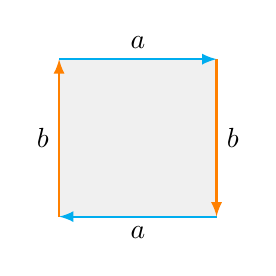
\begin{tikzpicture}
		\fill[fill=gray!12] (-1,-1) --(1,-1)--(1,1)--(-1,1)-- cycle;
		\draw [color=cyan,thick,-latex]  (1,-1)-- node [color=black,pos=0.5,below]{$a$} (-1,-1);
		\draw [color=orange,thick,-latex](-1,-1) -- node [color=black,pos=0.5,left]{$b$} (-1,1) ;
		\draw [color=orange,thick,-latex] (1,1)--node [color=black,pos=0.5,right]{$b$}(1,-1);
		\draw [color=cyan,thick,-latex] (-1,1)-- node [color=black,pos=0.5,above]{$a$} (1,1);
	\end{tikzpicture}
\end{center}
\subsection{Complex projective line $P^1(\mathbb{C})$}
Real projective line $P^1(\mathbb{R})$ is the set of equivalence classes of $\mathbb{R}^2-{(0,0)}$ under the equivalence relation $\sim$ defined by $x\sim y$ if there is a nonzero real number $\lambda$ such that $x = \lambda y$. We have the following homeomorphisms $P^1(\mathbb{C})\cong \mathbb{C}\cup\{\infty\}\cong \mathbb{R}^2\cup\{\infty\}\cong S^2$.
\subsection{Torus $T^2$}
A torus $T^2$ is a closed surface defined as the product of two circles $S^1 \times S^1$.
Torus can be described by a square with some edges identified as follows
\begin{center}
	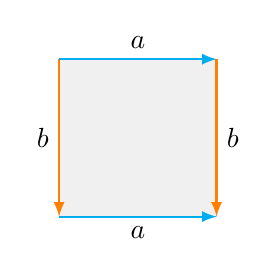
\begin{tikzpicture}
		\fill[fill=gray!12] (-1,-1) --(1,-1)--(1,1)--(-1,1)-- cycle;
		\draw [color=cyan,thick,-latex] (-1,-1) -- node [color=black,pos=0.5,below]{$a$} (1,-1);
		\draw [color=orange,thick,-latex] (-1,1)-- node [color=black,pos=0.5,left]{$b$}(-1,-1)  ;
		\draw [color=orange,thick,-latex] (1,1)--node [color=black,pos=0.5,right]{$b$}(1,-1);
		\draw [color=cyan,thick,-latex] (-1,1)-- node [color=black,pos=0.5,above]{$a$} (1,1);
	\end{tikzpicture}
\end{center}
\subsection{Möbius strip}
Möbius strip can be described by a square with some edges identified as follows
\begin{center}
	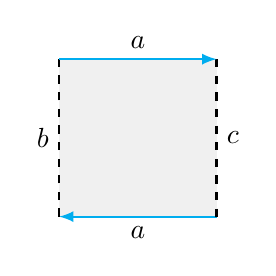
\begin{tikzpicture}
		\fill[fill=gray!12] (-1,-1) --(1,-1)--(1,1)--(-1,1)-- cycle;
		\draw [color=cyan,thick,-latex] (1,-1) -- node [color=black,pos=0.5,below]{$a$} (-1,-1);
		\draw [color=black,thick,dashed](-1,-1) -- node [color=black,pos=0.5,left]{$b$} (-1,1) ;
		\draw [color=black,thick,dashed] (1,1)--node [color=black,pos=0.5,right]{$c$}(1,-1);
		\draw [color=cyan,thick,-latex] (-1,1)-- node [color=black,pos=0.5,above]{$a$} (1,1);
	\end{tikzpicture}
\end{center}
\subsection{Klein bottle}

Klein bottle can be described by a square with some edges identified as follows
\begin{center}
	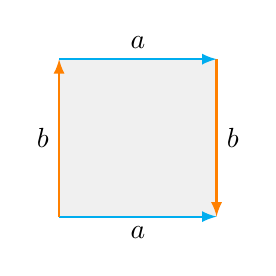
\begin{tikzpicture}
		\fill[fill=gray!12] (-1,-1) --(1,-1)--(1,1)--(-1,1)-- cycle;
		\draw [color=cyan,thick,-latex] (-1,-1) -- node [color=black,pos=0.5,below]{$a$} (1,-1);
		\draw [color=orange,thick,-latex](-1,-1) -- node [color=black,pos=0.5,left]{$b$} (-1,1) ;
		\draw [color=orange,thick,-latex] (1,1)--node [color=black,pos=0.5,right]{$b$}(1,-1);
		\draw [color=cyan,thick,-latex] (-1,1)-- node [color=black,pos=0.5,above]{$a$} (1,1);
	\end{tikzpicture}
\end{center}
\section{Other manifolds}
\subsection{Real projective space $P^n(\mathbb{R})$}
Real projective plane $P^n(\mathbb{R})=(\mathbb{R}^{n+1}-\{\mathbf{0}\})/\sim$ where $x\sim y$ whenever there is a nonzero real number $\lambda$ such that $x = \lambda y$. In general, we have
$$
	P^n(\mathbb{R})\cong S^n/\{\pm 1\}\cong D^n\sqcup (\partial D^n/{\pm 1})= D^n\sqcup (S^{n-1}/\{\pm 1\})\cong D^n\sqcup P^{n-1}(\mathbb{R})\cong \overline{D^n}\sqcup_{\partial D^n} P^{n-1}(\mathbb{R}),
$$
where $D^n:=\{x\in\mathbb{R}^{n+1}:\Vert x\Vert\le1\}$.

\chapter*{Appendix}

\begin{table}[h]
	\centering
	\begin{tblr}{
		colspec={|Q[m,c,1cm]|Q[m,c,1cm]|Q[m,c,1cm]|Q[m,c,0.8cm]|},
		row{1, 5} = {8ex},
		cell{1, 3, 5}{4} = {green7}}
		\hline
		\SetCell[r=5]{m} $\overline{A}$ & $A^\circ$                     & \SetCell[r=4]{m} $A'$ &\\ \cline{2-2} \cline{4-4}
		                                & \SetCell[r=4]{m} $\partial A$ &                       &\\ \cline{4-4}
		                                &                               &                       &\\ \cline{4-4}
		                                &                               &                       &\\ \cline{3-4}
		                                &                               & $A^s$                 &\\
		\hline
	\end{tblr}
\end{table}


\end{document}

